\section{Reducing the Chains-Division Problem to the Assignment Problem}
In this section, we will show how we can reduce the problem of finding the optimal partition of the nodes of a labeled tree $T$ given their equivalence classes into $p$ chains to the Minimum Weight Perfect Bipartite Matching problem (see \cref{def:mwpbm}). We define $\equivset$ as the set of equivalence classes of the nodes of $T$, and $t$ as the number of nodes of the tree. This reduction will allow us to solve the problem in polynomial time, as shown in the previous chapter.

In particular, we show that, given a tree $T$ and the number of chains $p$, we can construct a bipartite graph $G = (V, E)$ in which a perfect matching (\cref{def:matching}) always exists. In turn, a perfect matching with minimum weight enables us to retrieve the optimal partition of the nodes in $T$ into $p$ chains, such that the run-length encoding of each chain is minimized.

Then, we will show how to optimize the reduction by introducing some constraints that will allow us to reduce the number of edges in the bipartite graph, and we will also show how to move from the Minimum Weight Perfect Bipartite Matching problem to the more studied Maximum Weight Perfect Bipartite Matching problem without losing generality.

\subsection{Chains-Division Problem Definition}
It is essential to begin by defining the problem we aim to solve.

\begin{definition}[Chains-Division Problem] \label{def:problem_def}
    Given a labeled tree $T$, the equivalence classes $\equivset$, the stable order of the nodes in $T$ according to the upward path $\pi$ as defined in \cref{def:node_informations}, and an integer parameter $p \in [2, t]$, find the optimal partition of the nodes of $T$ into $p$ chains such that the run-length encoding of each chain is minimized.
\end{definition}

Let's give a formal definition of run-length encoding.
\begin{definition}[Run length encoding]
    Given a sequence $S = \{s_1, s_2, \dots, s_n\}$, the run length encoding of $S$ is the sequence $R = \{r_1, r_2, \dots, r_m\}$ where $r_i$ is the number of times the element $s_i$ is repeated in $S$.
\end{definition}

It allows us to represent the sequence $S$ in a more compact way. 

\begin{example}
    Let $S = \{A, A, B, B, B, C, C, A, A\}$. The run-length encoding of $S$ would be $R = \{(A, 2), (B, 3), (C, 2), (A, 2)\}$. The length of the RLE, which is the value we want to minimize, is $|R|=4$.
\end{example}

So, we aim to divide the nodes of the tree into $p$ chains such that the run-length encoding of the chains is minimized, meaning we want to reduce the number of distinct equivalence classes in each chain. Follows the definition of a chain.

\begin{definition}[Chains] \label{def:chains}
    Given a tree $T$, a chain $C$ is a sequence of nodes $C = \{c_1, c_2, \dots, c_m\}$ such that $C\subseteq V$. Additionally, each node of $T$ belongs to exactly one chain, and the nodes in the chain are ordered according to the upward path $\pi$ (as defined in \cref{def:node_informations}) of each node $c_i$.
\end{definition}

Note that, following the XBWT definition, two sibling nodes are comparable. The stable sorting algorithm respects the original sibling order, meaning the node that appears first among its siblings in a pre-order traversal will also come first in the sorted sequence.

\begin{example}[Chains-Division Problem]
    Consider a tree $T$ with 7 nodes having the following equivalence classes: $E = \{A, B, A, C, A, B, B\}$, where the nodes are ordered according to their upward paths. Let's say we want to divide these nodes into $p = 2$ chains.
    
    \textbf{Non-optimal division:} If we divide the nodes into chains $C_1 = \{A, B, A, C\}$ and $C_2 = \{A, B, B\}$, the run-length encoding would be:
    \begin{itemize}
        \item $C_1$: $(A,1), (B,1), (A,1), (C,1)$ - requiring 4 pairs
        \item $C_2$: $(A,1), (B,2)$ - requiring 2 pairs
    \end{itemize}
    Total RLE cost: $4 + 2 = 6$
    
    \textbf{Optimal division:} A better division would be $C_1 = \{A, A, A\}$ and $C_2 = \{B, C, B, B\}$, with run-length encoding:
    \begin{itemize}
        \item $C_1$: $(A,3)$ - requiring 1 pair
        \item $C_2$: $(B,1), (C,1), (B,2)$ - requiring 3 pairs
    \end{itemize}
    Total RLE cost: $1 + 3 = 4$
    
    This example demonstrates how grouping nodes of the same equivalence class in chains minimizes the total run-length encoding cost. The optimal solution can be found by reducing this problem to the \textsc{MWPBM} problem as described in this chapter.
\end{example}

\begin{comment}
\subsection{Reduction idea}
The intuition behind the reduction is the following: given a tree $T$ and the number of chains $p$, we can construct a bipartite graph $G = (V, E)$ in which a perfect matching (\cref{def:matching}) always exists. In turn, a perfect matching with minimum weight enables us to retrieve the optimal partition of the nodes in $T$ into $p$ chains, such that the run-length encoding of each chain is minimized.

In the following sections we will show how to construct the bipartite graph $G$ and proof that $G$ constructed as defined in \cref{def:bip_construction} always allows to find a perfect matching and the weight of the matching is the minimum run length encoding of the optimal partition of the nodes of $T$ into $p$ chains.

\alessio{Introduci il bipartite graph con troppa cattiveria :). Prima abbiamo parlato di alberi, adesso subito di grafi bipartiti. La soluzione con grafo bipartito è quella che hai voluto seguire tu, quindi dovresti introdurla più come una scelta implementativa, che come un dato di fatto. In breve, dovresti dimostrare qua che Chains-Div. si riduce al MWBGP, quindi sarebbe da girare un attimo l'ordine: Se abbiamo un grafo con un perfect matching allora possiamo ridurre il problema -> creiamo un grafo in questo modo -> contiene un perfect matching -> possiamo sempre fare la riduzione.} \davide{Ho aggiunto un paragrafo introduttivo.. può andare o intendevi proprio girare tutta la dimostrazione?}
\alessio{Se l'esistenza perfect matching è sufficiente a fare la riduzione, secondo me è meglio girare l'ordine delle dimostrazioni. Altrimenti, se per la riduzione ti servono le proprietà specifiche del grafo che hai creato allora va bene questo ordine. Pensandoci, puoi riportare questa discussione nell'intrduzione della sezione 6.2, mettendo qualcosa tipo ``In particular we show that, given a tree $T$ and the number of chains $p$, we can construct a bipartite ...'' tra i due paragrafi che ci sono già. (occhio alle frasi troppo lunghe).}
\end{comment}

\subsection{Bipartite Graph Construction}
Now, we will show how to construct a bipartite graph that allows us to solve the \textsc{CHAINS-DIVISION} problem.

\begin{definition}[Bipartite graph construction] \label{def:bip_construction}
    Let $T$ be a tree with $t$ nodes, and $p$ the number of chains we want to partition the nodes into. Let $\equivset$ be the set of equivalence classes of the nodes of $T$. We can construct a bipartite graph $G = (V, E)$ such that vertices are divided in two disjoint sets $V = V_1 \cup V_2$ in the following way:
    \begin{itemize}[leftmargin=25pt]
        \item $V_1$ contains $t + p$ nodes composed by $p$ source nodes $s_1, s_2, \dots, s_p$ (referred to collectively as $\sourceset$) followed by the $t$ elements (referred to collectively as $\treeset{1}$) of $\equivset$. The nodes in $V_1$ follow a strict ordering $s_1 \prec s_2 \prec \dots \prec s_p \prec u_1 \prec u_2 \prec \dots \prec u_t$, where $u_i$ are the tree nodes ordered according to the upward path $\pi$ as defined in \cref{def:node_informations}.
        \item $V_2$ contains $t + p$ nodes composed by the $t$ elements (referred to collectively as $\treeset{2}$) of $\equivset$ followed by $p$ destination nodes $d_1, d_2, \dots, d_p$ (referred to collectively as $\destset$). The nodes in $V_2$ follow a strict ordering $v_1 \prec v_2 \prec \dots \prec v_t \prec d_1 \prec d_2 \prec \dots \prec d_p$, where $v_i$ are the tree nodes ordered according to the upward path $\pi$ as defined in \cref{def:node_informations}.
    \end{itemize}

    Then the edges of the graph $G$ are constructed in the following way:
    \begin{enumerate}[leftmargin=25pt]
        \item The $\sourceset$ nodes are connected to the first $p$ nodes with distinct equivalence class in $V_2$, with weight $1$.
        \item Let $u_i \in \treeset{1}$. We define $\equivsetfunc{u_i}$ as the equivalence class of node $u_i$. For each node $u_i$, we construct the following edges:
        
        - For the first $p$ nodes $v_j \in \treeset{2}$ such that $j > i$ and $\equivsetfunc{v_j} \neq \equivsetfunc{u_i}$, we add an edge $(u_i, v_j)$ with weight $1$. If there are fewer than $p$ nodes in $V_2$ with distinct equivalence classes, we stop earlier.

        - Let $v_k \in \treeset{2}$ be the first node in the ordering such that $k > i$ and $\equivsetfunc{v_k} \neq \equivsetfunc{u_i}$, we add an edge $(u_i, v_k)$ with weight $0$. If such a node does not exist, we add $p$ edges $(u_i, d_j)$ with weight $0$ for each $j = 1, 2, \ldots, p$, where $d_j \in \destset$.
    \end{enumerate}
\end{definition}

Notice that it is important to consider the order of the nodes of the two sets $V_1$ and $V_2$ as stated in the definition, because we will need to connect the source nodes to the destination nodes in a way that will allow us to find the optimal partition of the nodes of the tree. An example of the node structure is shown in \cref{ex:reduction_vertices}.

Notice also that when we talk about the same $\treeset{1}$ node placed in $\treeset{2}$, we are referring to the corresponding node in $\treeset{2}$ that derives from the same node in the original tree $T$ since the nodes of the tree are ordered in both sets $\treeset{1}$ and $\treeset{2}$. In \cref{fig:bipartite_structure,fig:reduction_small_examples,fig:reduction_example}, the node's correspondence is achieved by putting the two nodes at the same level.
\begin{example}[Vertices] \label{ex:reduction_vertices}
    This example illustrates the structure of the bipartite graph vertices for the tree shown in \cref{fig:original_tree}. The nodes in this tree are labeled by their equivalence classes obtained from the minimization of the corresponding DAWG in \cref{ex:DAWG_minimization}. Our goal is to partition the tree's nodes into $p=2$ chains.

    \cref{fig:bipartite_structure} shows the corresponding bipartite graph. The graph is composed of:
    \begin{itemize}
        \item Two source nodes ($s_1, s_2$) on the left, representing the start of each chain.
        \item Two sets of tree nodes, representing the partitions $\treeset{1}$ (left column) and $\treeset{2}$ (right column). These nodes are ordered based on the \texttt{pathSort} algorithm. The labels (A, B, C, D) correspond to the equivalence classes from the original tree.
        \item Two destination nodes ($d_1, d_2$) on the right, representing the end of each chain.
    \end{itemize}

    % First figure - Original tree
    \begin{figure}[H]
        \centering
        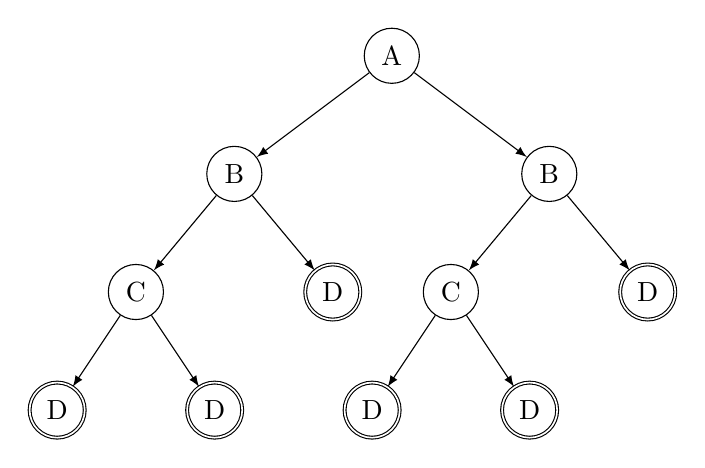
\begin{tikzpicture}[
            level distance=1.5cm,
            sibling distance=3cm,
            state/.style={circle, draw, minimum size=7mm},
            accepting/.style={circle, draw, double, minimum size=7mm},
            edge from parent/.style={draw, -latex},
            level 1/.style={sibling distance=4cm},
            level 2/.style={sibling distance=2.5cm},
            level 3/.style={sibling distance=2cm}
            ]
        
        \node[state] (a) {A}
            child {node[state] (b) {B} 
            child {node[state] (d) {C}
                child {node[accepting] (h) {D}}
                child {node[accepting] (i) {D}}
            }
            child {node[accepting] (e) {D}}
            }
            child {node[state] (c) {B}
            child {node[state] (f) {C}
                child {node[accepting] (l) {D}}
                child {node[accepting] (m) {D}}
            }
            child {node[accepting] (g) {D}}
            };
        \end{tikzpicture}
        \caption{Tree resulting from DAWG minimization of \cref{fig:example_dawg}. Each node is labeled with its equivalence class.}
        \label{fig:original_tree}
    \end{figure}
    
    % Second figure - Bipartite graph structure
    \begin{figure}[H]
        \centering
        \tikzset{main/.style = {draw, circle, thick, minimum size=8mm, inner sep=0pt}}
        \begin{tikzpicture}[node distance=10mm]
            % Define node styles
            \tikzstyle{main} = [circle, draw, minimum size=0.8cm, font=\small]
            \tikzstyle{source} = [circle, draw, minimum size=0.8cm, font=\small, fill=green!20]
            \tikzstyle{dest} = [circle, draw, minimum size=0.8cm, font=\small, fill=blue!20]
            
            % Source nodes (left column, green background)
            \node[source] (s1) {$s_1$};
            \node[source] (s2) [below of=s1] {$s_2$};
            
            % Tree nodes (left column, red border)
            \node[main] (t1) [below of=s2, yshift=-0.3cm] {A};
            \node[main] (t2) [below of=t1] {D};
            \node[main] (t3) [below of=t2] {D};
            \node[main] (t4) [below of=t3] {C};
            \node[main] (t5) [below of=t4] {D};
            \node[main] (t6) [below of=t5] {D};
            \node[main] (t7) [below of=t6] {D};
            \node[main] (t8) [below of=t7] {B};
            \node[main] (t9) [below of=t8] {B};
            \node[main] (t10) [below of=t9] {C};
            \node[main] (t11) [below of=t10] {D};
            
            % Tree nodes (right column, red border)
            \node[main] (r1) [right of=t1, xshift=3cm] {A};
            \node[main] (r2) [below of=r1] {D};
            \node[main] (r3) [below of=r2] {D};
            \node[main] (r4) [below of=r3] {C};
            \node[main] (r5) [below of=r4] {D};
            \node[main] (r6) [below of=r5] {D};
            \node[main] (r7) [below of=r6] {D};
            \node[main] (r8) [below of=r7] {B};
            \node[main] (r9) [below of=r8] {B};
            \node[main] (r10) [below of=r9] {C};
            \node[main] (r11) [below of=r10] {D};
            
            % Destination nodes (right column, blue background)
            \node[dest] (d1) [below of=r11, yshift=-0.3cm] {$d_1$};
            \node[dest] (d2) [below of=d1] {$d_2$};
            
            % Draw colored rectangles around groups
            % Green rectangle for source nodes
            \draw[green, thick, rounded corners] ([xshift=-0.4cm,yshift=0.25cm]s1.north west) rectangle ([xshift=0.4cm,yshift=-0.25cm]s2.south east);
            
            % Red rectangle for left tree nodes
            \draw[red, thick, rounded corners] ([xshift=-0.4cm,yshift=0.4cm]t1.north west) rectangle ([xshift=0.4cm,yshift=-0.4cm]t11.south east);
            
            % Red rectangle for right tree nodes
            \draw[red, thick, rounded corners] ([xshift=-0.4cm,yshift=0.4cm]r1.north west) rectangle ([xshift=0.4cm,yshift=-0.4cm]r11.south east);
            
            % Blue rectangle for destination nodes
            \draw[blue, thick, rounded corners] ([xshift=-0.4cm,yshift=0.25cm]d1.north west) rectangle ([xshift=0.4cm,yshift=-0.25cm]d2.south east);
            
            % Add labels
            \node[green!100, font=\small\bfseries] at ([xshift=1.5cm]s1.east) {Source};
            \node[green!100, font=\small\bfseries] at ([xshift=1.5cm]s2.east) {nodes};
            
            \node[red, font=\small\bfseries] at ([xshift=1.5cm]t6.east) {Tree};
            \node[red, font=\small\bfseries] at ([xshift=1.5cm]t7.east) {nodes};
            
            \node[blue, font=\small\bfseries] at ([xshift=-1.5cm]d1.west) {Destination};
            \node[blue, font=\small\bfseries] at ([xshift=-1.5cm]d2.west) {nodes};
            
            % Add "Corresponding tree node" label with arrow
            \draw[<->, thick] (t1.east) -- (r1.west);
            \node[font=\small] at ([xshift=0cm,yshift=-0.25cm]$(t1)!0.5!(r1)$) {Corresponding};
            \node[font=\small] at ([xshift=0cm,yshift=-0.7cm]$(t1)!0.5!(r1)$) {tree node};
            
        \end{tikzpicture}
        \caption{Corresponding bipartite graph structure for the tree in \cref{fig:original_tree} with $p=2$. The nodes are ordered from top to bottom using \cref{alg:pathSort}.}
        \label{fig:bipartite_structure}
    \end{figure}
\end{example}

\begin{example}[Edges]
    Let's see a small example for each case. Consider $p=2$. In \cref{fig:reduction_small_examples}-(a), there is an example for the sources' edges. As stated before, for each source, $p$ edges with weight $1$ are created and connected to the first $p$ nodes with distinct equivalence classes in $\treeset{2}$.

    In \cref{fig:reduction_small_examples}-(b), there is an example for the tree nodes' edges. For each node in $\treeset{1}$, edges with weight $1$ are created and connected to the first $p$ nodes with distinct equivalence class in $\treeset{2}$ after the corresponding node in $\treeset{2}$ (coming after the node itself in the ordering), and edges with weight $0$ are created and connected to the first node with the same class in $\treeset{2}$ after the corresponding node in $\treeset{2}$. As we can see from the image, we consider the first node in $\treeset{1}$ labelled $A$ that is connected to the node labelled $B$ with weight $1$, and to the node labelled $C$ with weight $1$, and to the second node labelled $A$ in $V_2$ with weight $0$.

    Lastly, in \cref{fig:reduction_small_examples}-(c) there is an example for the destination nodes' edges. We start by considering the node in $\treeset{1}$ that is labeled $A$, which is connected to a node labeled $B$ with weight $1$. Then, since there is no node with the same class in $\treeset{2}$, we connect it to the destination nodes $d_1$ and $d_2$ with weight $0$. The same is done for the second node in $V_1$ that is labelled $B$ since no nodes are coming after it in the order; it is connected to the destination nodes $d_1$ and $d_2$ with weight $0$.

    \begin{figure}[H]
        \centering
        \tikzset{main/.style = {draw, circle, thick, minimum size=8mm, inner sep=0pt}}
        \begin{subfigure}[b]{0.3\textwidth}
            \centering
            \begin{tikzpicture}[node distance=10mm, auto=center]
                \tikzstyle{main} = [circle, draw, minimum size=0.8cm, font=\small]
                \tikzstyle{source} = [circle, draw, minimum size=0.8cm, font=\small, fill=green!20]
                \tikzstyle{dest} = [circle, draw, minimum size=0.8cm, font=\small, fill=blue!20]
                
                % Left column (sources)
                \node[source] (1s) {$s_1$};
                \node[source] (2s) [below of=1s] {$s_2$};
                \node[main] (3s) [below of=2s] {A};
                \node[right=0cm of 3s] {$\cdots$};
                \node[main] (4s) [below of=3s] {A};
                \node[right=0cm of 4s] {$\cdots$};
                \node[main] (5s) [below of=4s] {B};
                \node[right=0cm of 5s] {$\cdots$};
                \node (dots_s) [below of=5s] {\vdots}; % Vertical dots

                % Right column (destinations)
                \node[main] (1d) [right=2.5cm of 3s] {A};
                \node[main] (2d) [below of=1d] {A};
                \node[left=0cm of 2d] {$\cdots$};
                \node[main] (3d) [below of=2d] {B};
                \node[left=0cm of 3d] {$\cdots$};
                \node (dots_d) [below of=3d] {\vdots}; % Vertical dots

                % Arrows
                \draw[red, ->] (1s) -- (1d);
                \draw[red, ->] (1s) -- (3d);
                \draw[red, ->] (2s) -- (1d);
                \draw[red, ->] (2s) -- (3d);
            \end{tikzpicture}
            \caption{}
            \label{fig:sub1}
        \end{subfigure}
        \hfill % Space between subfigures
        \tikzset{main/.style = {draw, circle, thick, minimum size=8mm, inner sep=0pt}}
        \begin{subfigure}[b]{0.3\textwidth}
            \centering
            \begin{tikzpicture}[node distance=10mm, auto=center]
                \tikzstyle{main} = [circle, draw, minimum size=0.8cm, font=\small]
                \tikzstyle{source} = [circle, draw, minimum size=0.8cm, font=\small, fill=green!20]
                \tikzstyle{dest} = [circle, draw, minimum size=0.8cm, font=\small, fill=blue!20]

                % Left column (tree nodes)
                \node (dots_s_top) {\vdots};
                \node[main] (3s) [below of=dots_s_top] {A};
                \node[main] (4s) [below of=3s] {B};
                \node[right=0cm of 4s] {$\cdots$};
                \node[main] (5s) [below of=4s] {A};
                \node[right=0cm of 5s] {$\cdots$};
                \node[main] (6s) [below of=5s] {C};
                \node[right=0cm of 6s] {$\cdots$};
                \node (dots_s_bottom) [below of=6s] {\vdots};

                % Right column (destinations)
                \node (dots_d_top) [right=2.5cm of dots_s_top] {\vdots};
                \node[main] (1d) [below of=dots_d_top] {A};
                \node[left=0cm of 1d] {$\cdots$};
                \node[main] (2d) [below of=1d] {B};
                \node[left=0cm of 2d] {$\cdots$};
                \node[main] (3d) [below of=2d] {A};
                \node[left=0cm of 3d] {$\cdots$};
                \node[main] (4d) [below of=3d] {C};
                \node[left=0cm of 4d] {$\cdots$};
                \node (dots_d_bottom) [below of=4d] {\vdots};

                % Arrows
                \draw[red, ->] (3s) -- (2d);
                \draw[red, ->] (3s) -- (4d);
                \draw[green, ->] (3s) -- (3d);
            \end{tikzpicture}
            \caption{}
            \label{fig:sub2}
        \end{subfigure}
        \hfill % Space between subfigures
        \tikzset{main/.style = {draw, circle, thick, minimum size=8mm, inner sep=0pt}}
        \begin{subfigure}[b]{0.3\textwidth}
            \centering
            \begin{tikzpicture}[node distance=10mm, auto=center]
                \tikzstyle{main} = [circle, draw, minimum size=0.8cm, font=\small]
                \tikzstyle{source} = [circle, draw, minimum size=0.8cm, font=\small, fill=green!20]
                \tikzstyle{dest} = [circle, draw, minimum size=0.8cm, font=\small, fill=blue!20]

                % Left column (original destinations)
                \node (dots_s_top) {\vdots};
                \node[main] (7s) [below of=dots_s_top] {A};
                \node[main] (9s) [below of=7s] {B};

                % Right column (bipartite graph destinations)
                \node (dots_d_top) [right=2.5cm of dots_s_top] {\vdots};
                \node[main] (5d) [below of=dots_d_top] {A};
                \node[left=0cm of 5d] {$\cdots$};
                \node[main] (6d) [below of=5d] {B};
                \node[left=0cm of 6d] {$\cdots$};
                \node[dest] (8d) [below of=6d] {$d_1$};
                \node[left=0cm of 8d] {$\cdots$};
                \node[dest] (9d) [below of=8d] {$d_2$};
                \node[left=0cm of 9d] {$\cdots$};

                % Arrows
                \draw[red, ->] (7s) -- (6d);
                \draw[green, ->] (7s) -- (8d);
                \draw[green, ->] (7s) -- (9d);
                \draw[green, ->] (9s) -- (8d);
                \draw[green, ->] (9s) -- (9d);
            \end{tikzpicture}
            \caption{}
            \label{fig:sub3}
        \end{subfigure}

        \caption[Examples of reduction to a bipartite graph]{Examples of the connection construction in the bipartite graph for $p=2$, showing the cases for source nodes $\sourceset$ (a), internal tree nodes $\treeset{1}$ and $\treeset{2}$ (b), and destination nodes $\destset$ (c). Red arrows indicate edges with weight 1, while green arrows indicate edges with weight 0.}
        \label{fig:reduction_small_examples}
    \end{figure}
\end{example}


Before we present the proof of the correctness of the reduction, let us state the following theorem regarding the number of edges in the bipartite graph resulting from \cref{def:bip_construction}. This theorem is essential for understanding the complexity of the final algorithm employed to solve the \textsc{MWPBM} problem and so, the \textsc{CHAIN-DIVISION} problem.

\begin{theorem}[Bipartite graph properties]
    The bipartite graph $G$ constructed as stated in \cref{def:bip_construction} has $2t + 2p$ nodes and $O(t (p + 1) + p^2 + tp)$ edges.
\end{theorem}

\begin{proof}
    The $O(t (p + 1))$ edges come from the tree nodes, the $O(p^2)$ edges come from the sources since each source node is connected to $p$ nodes, and the $O(tp)$ edges come from the destination nodes since in the worst case we have $t$ distinct equivalence classes meaning that all the nodes are connected to the destination nodes. 
\end{proof}

\subsection{Proof of Correctness}
In this section, we present the proof of the correctness of the reduction introduced in the previous sections. Let's start by stating the following lemmas.

\begin{comment}
\begin{lemma} \label{lemma:all_destinations}
    Exactly $|\equivset|$ nodes of the set $\treeset{1}$ are connected to all the destination nodes $d_i \in \destset$ with weight $0$.
\end{lemma}

\begin{proof}
    As outlined in \cref{def:bip_construction}, the destination nodes $d_i \in V_2$ are connected to nodes $u_i \in \treeset{1}$ with weight $0$ iff for all $v_j \in \treeset{2}$ such that $j > i$, $\equivsetfunc{v_j} \neq \equivsetfunc{u_i}$, i.e. $u_i$ is the last of its class in the ordering. Consequently, there are exactly $|\equivset|$ nodes in $\treeset{1}$ that are last representatives of their class in the ordering.
\end{proof}
\end{comment}

\begin{lemma} \label{lemma:optimal_cost}
    The optimal solution of an instance $\mathcal{I}$ of the \textit{CHAINS-DIVISION} problem for a tree $T$ is always greater than or equal to $|\equivset|$.
\end{lemma}

\begin{proof}
    To minimize the run-length encoding of the chains, we note that the minimum cost of a chain is $1$. Consequently, the optimal cost of the \textit{CHAINS-DIVISION} problem for the tree $T$ is always greater than or equal to the cardinality of the set of equivalence classes $\equivset$ This is because if we partition them into $p = |\equivset|$ chains, the cost will be equal to $|\equivset|$, since each chain contains only nodes belonging to the same class. Conversely, if we partition them into $p < |\equivset|$ chains, the cost will be greater than or equal to $|\equivset|$ since we will need to include at least two nodes from different classes within a single chain.
\end{proof}

\begin{claim} \label{claim:p_less_than_E}
    The solutions for the \textit{CHAINS-DIVISION} problem for the instances where the number $p$ of chains is greater than $|\equivset|$ are not better than the solutions for the instances where $p \leq |\equivset|$.
\end{claim}

\begin{proof}
    The proof builds upon \cref{lemma:optimal_cost}. If we use a number of chains $p > |\equivset|$, we would have at least $p - |\equivset|$ empty chains, since there are only $|\equivset|$ non-empty equivalence classes of nodes to partition. As the minimum cost for any chain is 1, these empty chains contribute to the total cost. An optimal arrangement would involve $|\equivset|$ chains, each containing nodes from a single equivalence class, costing $|\equivset|$, and $p - |\equivset|$ empty chains, each costing 1. The total cost would be $|\equivset| + (p - |\equivset|) = p$. Since $p > |\equivset|$, this cost is greater than the optimal cost of $|\equivset|$ achievable with $p = |\equivset|$ chains. Therefore, any solution with $p > |\equivset|$ is suboptimal.
\end{proof}

Therefore, for the proof of the reduction, we will only consider instances of the problem where $p < |\equivset|$, as they do not present a trivial solution.

\begin{lemma} \label{lemma:greater_nodes}
    Given a bipartite graph $G$ constructed as stated in \cref{def:bip_construction}, for each node $u_i \in$ $\treeset{1}$ it is impossible for $u_i$ to be connected to a node $v_j \in \treeset{2}$, such that $j \leq i$ in the order of the nodes.
\end{lemma}

\begin{proof}
    The proof comes from the construction of $G$ (\cref{def:bip_construction}) where the nodes of $\treeset{1}$ are always connected to the nodes of $\treeset{2}$ coming after them.
\end{proof}

\begin{lemma} \label{claim:node_connectivity}
    In the bipartite graph $G$ constructed as per \cref{def:bip_construction}, for every node $u \in \treeset{1}$ $|N(\{u\})| \geq 1$.
\end{lemma}
In other words, every node in $V_1$ is connected to at least another node in $V_2$.
\begin{proof}
    Let $u_i \in \treeset{1}$ be an arbitrary node. We analyze the construction of its outgoing edges based on \cref{def:bip_construction}. There are two mutually exclusive cases for $u_i$:
    \begin{enumerate}[leftmargin=25pt]
        \item There exists at least one node $v_k \in \treeset{2}$ with $k > i$ that has the same equivalence class as $u_i$, i.e., $\equivsetfunc{v_k} = \equivsetfunc{u_i}$. In this case, the construction specifies that an edge is added between $u_i$ and the first such node $v_k$. This guarantees $u_i$ has at least one neighbor.
        \item There are no nodes $v_k \in \treeset{2}$ with $k > i$ that share the same equivalence class as $u_i$. This occurs when $u_i$ is the last node of its equivalence class in the specified ordering. In this scenario, the construction adds $p$ edges from $u_i$ to each of the destination nodes $d_j \in \destset$. Since $p \geq 2$, $u_i$ is connected to at least two nodes.
    \end{enumerate}
    In either case, any node $u_i \in \treeset{1}$ is guaranteed to have at least one outgoing edge. Therefore, its neighborhood is non-empty.
\end{proof}

\begin{lemma} \label{lemma:distinct_neighborhoods}
    For any pair of distinct nodes $u_i, u_j \in \treeset{1}$ such that $u_i \prec u_j$, $N(\{u_i\}) \not\subseteq N(\{u_j\})$.
\end{lemma}
\begin{proof}
    By \cref{claim:node_connectivity}, the set of neighbors $N(\{u_i\})$ and $N(\{u_j\})$ are non-empty. We will show that $N(\{u_i\}) \not\subseteq N(\{u_j\})$. 
    
    By construction, $u_i$ is connected to $v_{i+1}$. This holds whether $v_{i+1}$ is the next node in the same equivalence class or one of the first $p$ nodes in a different class. Thus, $v_{i+1} \in N(\{u_i\})$.

    From \cref{lemma:greater_nodes}, any neighbor $v_k$ of $u_j$ must have $k > j$. Since $i < j$, we have $i+1 \leq j$.
    This means $v_{i+1}$ cannot be a neighbor of $u_j$, as $i + 1 < k$. Therefore, $v_{i+1} \in N(\{u_i\})$ but $v_{i+1} \notin N(\{u_j\})$, which proves that $N(\{u_i\}) \not\subseteq N(\{u_j\})$.
\end{proof}

\begin{lemma} \label{lemma:distinct_neighborhoods_2}
    For any pair of distinct nodes $u_i, u_j \in \treeset{1}$ such that $u_i \prec u_j$ and $u_j$ is not the last node of its equivalence class in the order, then $N(\{u_j\}) \not\subseteq N(\{u_i\})$.
\end{lemma}
\begin{proof}
    Since $u_j$ is not the last node of its equivalence class, by construction, it must be connected to the first node $v_k \in \treeset{2}$ with $k > j$ such that $\equivsetfunc{v_k} = \equivsetfunc{u_j}$. Therefore, $v_k \in N(\{u_j\})$.

    By construction, it follows that $u_i$ cannot be connected to $v_k$. This is due to the existence of another node $v_l \in \treeset{2}$ with $i < l \leq j$, such that $\equivsetfunc{v_l} = \equivsetfunc{u_k}$. Consequently, we conclude that $v_k \notin N(\{u_i\})$, as the edges of $u_i$ connect to nodes in $\treeset{2}$, all of which belong to distinct classes.

    In summary, we have identified a node $v_k$ that is included in $N({u_j})$ but excluded from $N({u_i})$, thus proving that $N({u_j}) \not\subseteq N({u_i})$.
\end{proof}

\begin{comment}
\alessio{Non so se sia abbastanza questo claim, forse andrebbe dimostrato in entrambe le direzioni, quindi $N(\{u_i\}) \not\subseteq N(\{u_j\})$ e $N(\{u_j\}) \not\subseteq N(\{u_i\})$. In pratica la dimostrazione è la stessa ma va spiegata bene. A questo punto no so se il Lemma 4 serva, dato che deriva fa questa proprietà. Quindi in pratica il nodo sopra sarà connesso a nodi sopra il nodo sotto, mentre il nodo sotto sarà connesso ad altri nodi più sotto.
Dimostrando questo, puoi dire che ogni nodo aggiunge sempre almeno un nodo in più a $N(W)$, che sarà quindi almeno uguale a $|W|$. Occhio che però questo vale solo per i nodi che non sono gli ultimi della loro classe.} \davide{dovrei aver dimostrato le due strade e aggiunto nel lemma dell'esistenza del matching il caso in cui $u_j$ è l'ultimo nodo della sua classe.}
\begin{claim} \label{claim:prev_not_subset}
    For any pair of distinct nodes $u_i, u_j \in \treeset{1}$ with $i < j$, then we have that $N(\{u_i\}) \not\subseteq N(\{u_j\})$.
\end{claim}
\begin{proof}
    This is a direct consequence of the proof of \cref{lemma:distinct_neighborhoods}. In its proof, we showed that for any pair of nodes $u_i, u_j$ with $i < j$, there exists a neighbor $v_k \in N(\{u_i\})$ such that $k \leq j$. By \cref{lemma:greater_nodes}, any neighbor of $u_j$ must have an index greater than $j$. Therefore, $v_k$ cannot be a neighbor of $u_j$, which implies that $N(\{u_i\})$ cannot be a subset of $N(\{u_j\})$.
\end{proof}
\end{comment}

\begin{lemma} \label{lemma:matching_existence}
    For every possible instance of the \textit{CHAINS-DIVISION} problem, a perfect matching exists in the bipartite graph G constructed as specified in \cref{def:bip_construction}.
\end{lemma}
\begin{proof}
    The proof comes from the construction of the bipartite graph $G$ and from \cref{thm:halls_marriage_theorem}. We are going to prove that $G$ satisfies Hall's condition (see \cref{thm:halls_marriage_theorem}) and so, since by construction $|V_1| = |V_2|$, a perfect matching for $G$ exists.

    To verify Hall's condition, we need to prove that for any subset $W \subseteq V_1$ we have that $|N(W)| \geq |W|$, where $N(W)$ is the neighborhood of $W$ (\cref{def:neighborhood}). We have the following cases:
    \begin{enumerate}[leftmargin=25pt]
        \item $W \subseteq \sourceset$: Let $W$ be a subset of $S$ of size $k$. By construction, every source node $s_i \in \sourceset$ is connected to the same set of $p$ nodes in $V_2$, which are the first $p$ nodes with distinct equivalence classes in the ordering. Therefore, for any non-empty $W \subseteq \sourceset$, the neighborhood $N(W)$ consists of exactly these $p$ nodes, so $|N(W)| = p$. From \cref{lemma:optimal_cost} and \cref{claim:p_less_than_E}, we only consider instances where $p \leq |\equivset|$, ensuring that at least $p$ such nodes exist. Since $|\sourceset|=p$, we have $|W| = k \leq p$. Thus, $|N(W)| \geq |W|$.
        
        \item $W \subseteq \treeset{1}$: Let $W = \{u_{i_1}, \dots, u_{i_k}\} \subseteq \treeset{1}$ with $i_1 < i_2 < \dots < i_k$. We analyze two subcases:

        \textbf{Case A: No node in $W$ is the last of its class.}
        By \cref{lemma:distinct_neighborhoods,lemma:distinct_neighborhoods_2}, for any two nodes $u_a, u_b \in W$ with $a < b$, we have both $N(\{u_a\}) \not\subseteq N(\{u_b\})$ and $N(\{u_b\}) \not\subseteq N(\{u_a\})$. This implies that each node in $W$ contributes at least one unique neighbor to the total neighborhood $N(W)$. Therefore, $|N(W)| \geq |W|$.

        \textbf{Case B: At least one node in $W$ is the last of its class.}
        Let $u_{j} \in W$ be a node that is the last of its equivalence class. By construction, $u_{j}$ is connected to all $p$ destination nodes $\destset$, which means $\destset \subseteq N(W)$ and thus $|N(W)| \geq p$.

        For such a node $u_j$, its neighborhood $N(\{u_j\})$ may be a subset of $N(\{u_a\})$ for some $u_a \in W$ with $a < j$, since \cref{lemma:distinct_neighborhoods_2} does not apply. However, the reverse is not true, as \cref{lemma:distinct_neighborhoods} guarantees $N(\{u_a\}) \not\subseteq N(\{u_j\})$. This asymmetry ensures that $N(\{u_a\})$ always contributes at least one neighbor not present in $N(\{u_j\})$. This property, combined with the fact that all nodes that are last of their class are connected to the $p$ destination nodes, is sufficient to guarantee that $|N(W)| \ge |W|$ since $p \geq 2$.

        In both cases, Hall's condition $|N(W)| \geq |W|$ is satisfied for any $W \subseteq \treeset{1}$.
        
        \item $W=W_S \cup W_U$, where $W_S \subseteq \sourceset, W_U \subseteq \treeset{1}$: The neighborhood of $W_S$ consists of $p$ nodes, as established in case 1 ($W \subseteq \sourceset$). By \cref{lemma:greater_nodes}, the neighbors of any node in $W_U$ appear later in the node ordering than the node itself. Since all nodes in $\treeset{1}$ are ordered after the source nodes, the neighbors of $W_U$ are distinct from the neighbors of $W_S$. Specifically, $N(W_S)$ consists of the first $p$ nodes with distinct equivalence classes.
        
        We now analyze two subcases for nodes in $W_U$: If $W_U$ contains a node $u_i \in \treeset{1}$ that is not the last of its equivalence class, then there exists at least one node $v_j \in \treeset{2}$ with $i < j$ and $\equivsetfunc{u_i} = \equivsetfunc{v_j}$ that is connected to $u_i$ but not to any source node. This contributes additional neighbors to $N(W)$, ensuring $|N(W)| \geq |W|$.
        If $W_U$ contains a node $u_i \in \treeset{1}$ that is the last of its equivalence class, then by construction, $u_i$ is connected to all destination nodes. This guarantees $|N(W)| \geq |W|$.
        
        In both subcases, Hall's condition $|N(W)| \geq |W|$ is satisfied.
    \end{enumerate}
\end{proof}

\begin{comment}
    \begin{proof}
        The proof comes from the construction of the bipartite graph $G$ and from \cref{thm:perfect_matching_existence}. We are going to prove that the bipartite graph $G$ constructed as stated in \cref{def:bip_construction} has a Tutte matrix (\cref{def:tutte_matrix}) with determinant different from $0$ and so a perfect matching for $G$ exists.

        We know that an $n \times n$ matrix $M$ has $Det(M) \neq 0$ if and only if it has full rank ($rank(M) = n$), or equivalently if it has $n$ linearly independent rows or columns. We can see that the bipartite graph $G$ has $2t + 2p$ nodes and $O(t (p + 1) + p^2 + tp)$ edges, and so the Tutte matrix of $G$ will have $2t + 2p$ rows and $2t + 2p$ columns. The columns of $M$ are all independent since each node of $G$ in $V_1$ is connected only to nodes in $V_2$ that are greater than $u$ in the ordering. Also, each node is connected to at least one node in $V_2$ and at most $p + 1$ distinct nodes with distinct class in $V_2$. Those conditions on the edges are sufficient to get a full rank matrix and so a perfect matching for $G$ exists.
    \end{proof}

    In \cref{fig:tutte_matrix_ex}, the Tutte matrix for the bipartite graph in \cref{fig:reduction_example}-(a) is shown.

    \begin{figure}
        \centering
        \[
        \begin{array}{c|ccccccccc}
                & \text{1} & \text{2} & \text{1} & \text{3} & \text{1} & \text{2} & \text{2} & \text{$d_1$} & \text{$d_2$} \\
            \hline
            \text{$s_1$} & 1 & 1 & 0 & 0 & 0 & 0 & 0 & 0 & 0 \\
            \text{$s_2$} & 1 & 1 & 0 & 0 & 0 & 0 & 0 & 0 & 0 \\
            \text{1}     & 0 & 1 & 1 & 1 & 0 & 0 & 0 & 0 & 0 \\
            \text{2}     & 0 & 0 & 1 & 1 & 0 & 1 & 0 & 0 & 0 \\
            \text{1}     & 0 & 0 & 0 & 1 & 1 & 1 & 0 & 0 & 0 \\
            \text{3}     & 0 & 0 & 0 & 0 & 1 & 1 & 0 & 1 & 1 \\
            \text{1}     & 0 & 0 & 0 & 0 & 0 & 1 & 0 & 1 & 1 \\
            \text{2}     & 0 & 0 & 0 & 0 & 0 & 0 & 1 & 0 & 0 \\
            \text{2}     & 0 & 0 & 0 & 0 & 0 & 0 & 0 & 1 & 1 \\
        \end{array}
        \]
        \caption[Tutte matrix example]{Example of a Tutte matrix for a bipartite graph in \cref{fig:reduction_example}-(a). As we can see the matrix has full rank and so a perfect matching exists.}
        \label{fig:tutte_matrix_ex}
    \end{figure}
\end{comment}

We can now prove the correctness of the reduction. Consider a perfect matching $M$ in $G$. Therefore, $|V_1|=|V_2|$ and $M$ is perfect, every node in $V_1$ is matched to exactly one node in $V_2$, and vice versa. The matching $M$ consists of $t+p$ edges. Due to the construction of $G$ (\cref{def:bip_construction}) and \cref{lemma:greater_nodes} (a node $u_i \in \treeset{1}$ only connect to a node $v_j \in \treeset{2}$ with $i < j$ or to destination nodes $\destset$), the matching $M$ naturally decomposes into $p$ paths starting from the source nodes $s_1, \dots, s_p$ and ending at the destination nodes $d_1, \dots, d_p$. Each path traverses a sequence of nodes corresponding to the nodes of the original tree $T$.
Specifically, a path starting at $s_i$ will match it to a node $u_{a} \in \treeset{2}$. Then, the corresponding node of $u_{a} \in \treeset{1}$ can be matched to a node $u_{b} \in \treeset{2}$ (where $b > a$). This continues until a node $u_{x} \in \treeset{1}$ is matched to a destination node $d_k \in \destset$. This forms a sequence $s_i \rightarrow u_{a} \rightarrow u_{b} \rightarrow \dots \rightarrow u_{x} \rightarrow d_k$. Following this technique, we will retrieve all the optimal chains from the solution of the \textsc{MWPBM} problem.

\begin{example}
    Consider the example in \cref{fig:example_bipartite_read}. It shows a bipartite graph constructed from a tree (not shown) and a perfect matching within it. The solid arrows represent the edges of the perfect matching, where an edge $(u, v)$ signifies that node $v$ follows node $u$ in a path. The dashed arrows link the segments of the paths by connecting a node's representation in $V_2$ to its corresponding representation in $V_1$.

    The matching partitions the nodes into two distinct paths, differentiated by color:
    \begin{itemize}
        \item \textbf{Path 1 (red):} Starting from source $s_1$, the matching edge $(s_1, A)$ leads to the first node, $A$. The dashed arrow from this node in $V_2$ points to the same node $A$ in $V_1$, which is then matched with another $A$ in $V_2$. Following the next dashed arrow to the final $A$ in $V_1$, we see it is matched with the destination $d_1$. This sequence traces the path $s_1 \to A \to A \to d_1$ leading to the chain $C_{red}=\{A,A\}$.
        \item \textbf{Path 2 (blue):} Starting from source $s_2$, the matching edge $(s_2, B)$ leads to node $B$. The dashed arrow connects to the next $B$ in $V_1$, which is matched with destination $d_2$, tracing the path $s_2 \to B \to d_2$ leading to the chain $C_{blue}=\{B\}$.
    \end{itemize}
    This demonstrates how a perfect matching in the bipartite graph yields a valid partition of the original tree's nodes into paths from sources to destinations.
    \begin{figure}[H]
        \centering
        \tikzset{main/.style = {draw, circle, thick, minimum size=8mm, inner sep=0pt}}
        \begin{tikzpicture}[node distance=10mm, auto=center]
            \tikzstyle{main} = [circle, draw, minimum size=0.8cm, font=\small]
            \tikzstyle{source} = [circle, draw, minimum size=0.8cm, font=\small, fill=green!20]
            \tikzstyle{dest} = [circle, draw, minimum size=0.8cm, font=\small, fill=blue!20]

            % Left column (original destinations)
            \node[source] (1s) {$s_1$};
            \node[source] (2s) [below of=1s] {$s_2$};
            \node[main] (7s) [below of=2s] {A};
            \node[main] (8s) [below of=7s] {A};
            \node[main] (9s) [below of=8s] {B};

            % Right column (bipartite graph destinations)
            \node[main] (5d) [right=2.5cm of 7s] {A};
            \node[main] (7d) [below of=5d] {A};
            \node[main] (6d) [below of=7d] {B};
            \node[dest] (8d) [below of=6d] {$d_1$};
            \node[dest] (9d) [below of=8d] {$d_2$};

            % Arrows
            \draw[red, ->] (1s) -- (5d);
            \draw[red, ->] (7s) -- (7d);
            \draw[red, ->] (8s) -- (8d);
            \draw[red, dashed, ->] (5d) -- (7s);
            \draw[red, dashed, ->] (7d) -- (8s);

            \draw[blue, ->] (2s) -- (6d);
            \draw[blue, ->] (9s) -- (9d);
            \draw[blue, dashed, ->] (6d) -- (9s);
        \end{tikzpicture}
        \caption{An example of a perfect matching (solid lines) in the constructed bipartite graph. The matching defines a partition into two paths (red and blue), which are traced by following the solid and dashed arrows.}
        \label{fig:example_bipartite_read}
    \end{figure}
\end{example}

\begin{theorem}
    An optimal solution of an instance $\mathcal I$ with $p \leq |\equivset|$ of the \textsc{CHAINS-DIVISION} problem (\cref{def:problem_def}) is equivalent to an optimal solution of the \textsc{MWPBM} problem (\cref{def:mwpbm}) for the instance $r(\mathcal I)$ where $r: \mathcal{I}_{CHAINS-DIVISION} \rightarrow \mathcal{I}_{MWPBM}$ is the reduction function that maps an instance of the CHAINS-DIVISION problem to an instance of the MWPBM problem for a bipartite graph $G$ constructed as stated in \cref{def:bip_construction}.
\end{theorem}

\begin{proof}
    Let $\mathcal{I} = (T, \equivset, p)$ be an instance of the \textsc{CHAINS-DIVISION} problem, where $T$ is a tree with $t$ nodes, $\equivset$ is the set of equivalence classes, and $p$ is the target number of chains. We assume $p \leq |\equivset|$, per \cref{claim:p_less_than_E}. Let $G = r(\mathcal{I})$ be the bipartite graph constructed according to \cref{def:bip_construction}. We will demonstrate a bijection between the set of valid chain partitions of $T$ and the set of perfect matchings in $G$, such that the cost of a partition equals the weight of its corresponding matching.

    First, we establish the existence of a perfect matching. By construction, the graph $G$ is bipartite with partitions $V_1$ and $V_2$ such that $|V_1| = |V_2| = t+p$. \cref{lemma:matching_existence} ensures that a perfect matching exists in $G$.

    Let $\mathcal{P} = \{C_1, \dots, C_p\}$ be a valid partition of the nodes of $T$ into $p$ chains. We can construct a perfect matching $M_\mathcal{P}$ in $G$ as follows:  For each chain $C_k = [u_{1}, \dots, u_{m_k}]$, we construct a path in $G$: match $s_k$ to $u_{1} \in \treeset{2}$. Then match $u_{i} \in \treeset{1}$ to $u_{i+1} \in \treeset{2}$ for $i=1, \dots, m_k-1$. Finally, match $u_{m_k} \in \treeset{1}$ to one of the available destination nodes $d_j \in \destset$. Since we have $p$ chains and $p$ source/destination nodes, and every tree node is in exactly one chain, this process uses all $t+p$ nodes in $V_1$ and $V_2$, forming a perfect matching. The weight of this matching is given by:
    \begin{align*}
        W(M_\mathcal{P}) &= \sum_{(u,v) \in M_\mathcal{P}} w(u,v) \\
        &= p + |\{ (u_i, u_j) \in M_\mathcal{P} \mid u_i \in \treeset{1}, u_j \in \treeset{2}, \equivsetfunc{u_i} \neq \equivsetfunc{u_j} \}|
    \end{align*}
    where $p$ represents the contribution from the source nodes $s_i$, as each source node must be connected with weight 1 to start a chain. A class change occurs exactly when a path in the matching uses a weight-1 edge between tree nodes.
    Therefore, $W(M)$ is exactly equal to the RLE cost of the partition defined by the matching $M_\mathcal{P}$.

    Conversely, let $M$ be a perfect matching in $G$. The structure of $G$ ensures that $M$ consists of $p$ disjoint paths starting from source nodes $\{s_1, \dots, s_p\}$ and ending at destination nodes $\{d_1, \dots, d_p\}$. Each path defines an ordered chain of nodes from $T$. By \cref{lemma:greater_nodes}, the node order within these chains is consistent with the original node ordering $\pi$. Thus, $M$ maps to a valid partition of $T$. The cost of this partition is equal to $W(M)$.

    Since there is a cost-preserving bijection between the set of all valid partitions and the set of all perfect matchings, an optimal solution to one problem corresponds to an optimal solution to the other. Therefore, finding a minimum weight perfect matching in $G$ is equivalent to solving the \textsc{CHAINS-DIVISION} problem for $T$.
\end{proof}

\begin{example}
    Consider the example in \cref{fig:reduction_example} where we have the bipartite graph for the tree in \cref{fig:original_tree} and $p = 2$. In \cref{fig:reduction_example}-(a) we have the resulting bipartite graph, and in \cref{fig:reduction_example}-(b) we have one of the possible minimum perfect matchings for the graph in (a) having weight $5$. At the end we can see that the optimal partition of the nodes of the tree $T$ is $C_1 = \{A,C,B,B,C\}$ and $C_2 = \{D,D,D,D,D,D\}$ with a total cost of $5$, this can be obtained starting from the sources and by following the edges of the nodes, jumping to the corresponding node in $V_1$ and following the edges again until we reach the destination nodes.

    \begin{figure}[H]
        \centering
        \begin{tabular}{cc}
            \tikzset{main/.style = {draw, circle, thick, minimum size=8mm, inner sep=0pt}}
            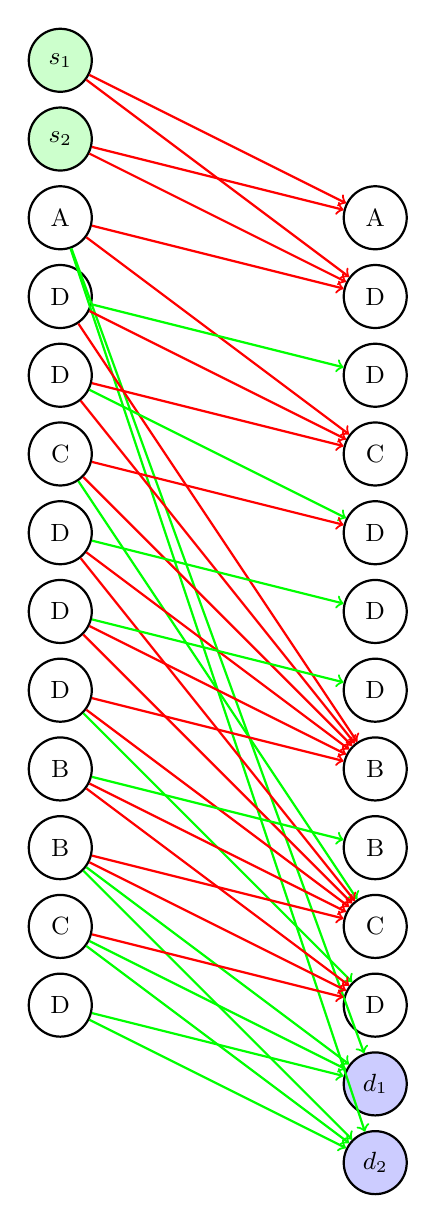
\begin{tikzpicture}[node distance={10mm}, thick, auto=center, main/.style = {draw, circle}]
                \tikzstyle{main} = [circle, draw, minimum size=0.8cm, font=\small]
                \tikzstyle{source} = [circle, draw, minimum size=0.8cm, font=\small, fill=green!20]
                \tikzstyle{dest} = [circle, draw, minimum size=0.8cm, font=\small, fill=blue!20]

                % Source nodes (left column, green background)
                \node[source] (s1) {$s_1$};
                \node[source] (s2) [below of=s1] {$s_2$};
                
                % Tree nodes (left column, red border)
                \node[main] (t1) [below of=s2] {A};
                \node[main] (t2) [below of=t1] {D};
                \node[main] (t3) [below of=t2] {D};
                \node[main] (t4) [below of=t3] {C};
                \node[main] (t5) [below of=t4] {D};
                \node[main] (t6) [below of=t5] {D};
                \node[main] (t7) [below of=t6] {D};
                \node[main] (t8) [below of=t7] {B};
                \node[main] (t9) [below of=t8] {B};
                \node[main] (t10) [below of=t9] {C};
                \node[main] (t11) [below of=t10] {D};
                
                % Tree nodes (right column, red border)
                \node[main] (r1) [right of=t1, xshift=3cm] {A};
                \node[main] (r2) [below of=r1] {D};
                \node[main] (r3) [below of=r2] {D};
                \node[main] (r4) [below of=r3] {C};
                \node[main] (r5) [below of=r4] {D};
                \node[main] (r6) [below of=r5] {D};
                \node[main] (r7) [below of=r6] {D};
                \node[main] (r8) [below of=r7] {B};
                \node[main] (r9) [below of=r8] {B};
                \node[main] (r10) [below of=r9] {C};
                \node[main] (r11) [below of=r10] {D};
                
                % Destination nodes (right column, blue background)
                \node[dest] (d1) [below of=r11] {$d_1$};
                \node[dest] (d2) [below of=d1] {$d_2$};
                
                \draw[red, ->] (s1) -- (r1);
                \draw[red, ->] (s1) -- (r2);
                \draw[red, ->] (s2) -- (r1);
                \draw[red, ->] (s2) -- (r2);
                \draw[red, ->] (t1) -- (r2);
                \draw[red, ->] (t1) -- (r4);
                \draw[green, ->] (t1) -- (d1);
                \draw[green, ->] (t1) -- (d2);
                \draw[green, ->] (t2) -- (r3);
                \draw[red, ->] (t2) -- (r4);
                \draw[red, ->] (t2) -- (r8);
                \draw[red, ->] (t3) -- (r4);
                \draw[red, ->] (t3) -- (r8);
                \draw[green, ->] (t3) -- (r5);
                \draw[red, ->] (t4) -- (r5);
                \draw[red, ->] (t4) -- (r8);
                \draw[green, ->] (t4) -- (r10);
                \draw[red, ->] (t5) -- (r8);
                \draw[red, ->] (t5) -- (r10);
                \draw[green, ->] (t5) -- (r6);
                \draw[red, ->] (t6) -- (r8);
                \draw[red, ->] (t6) -- (r10);
                \draw[green, ->] (t6) -- (r7);
                \draw[red, ->] (t7) -- (r8);
                \draw[red, ->] (t7) -- (r10);
                \draw[green, ->] (t7) -- (r11);
                \draw[red, ->] (t8) -- (r11);
                \draw[red, ->] (t8) -- (r10);
                \draw[green, ->] (t8) -- (r9);
                \draw[red, ->] (t9) -- (r11);
                \draw[red, ->] (t9) -- (r10);
                \draw[green, ->] (t9) -- (d1);
                \draw[green, ->] (t9) -- (d2);
                \draw[red, ->] (t10) -- (r11);
                \draw[green, ->] (t10) -- (d1);
                \draw[green, ->] (t10) -- (d2);
                \draw[green, ->] (t11) -- (d1);
                \draw[green, ->] (t11) -- (d2);
            \end{tikzpicture} &
            \tikzset{main/.style = {draw, circle, thick, minimum size=8mm, inner sep=0pt}}
            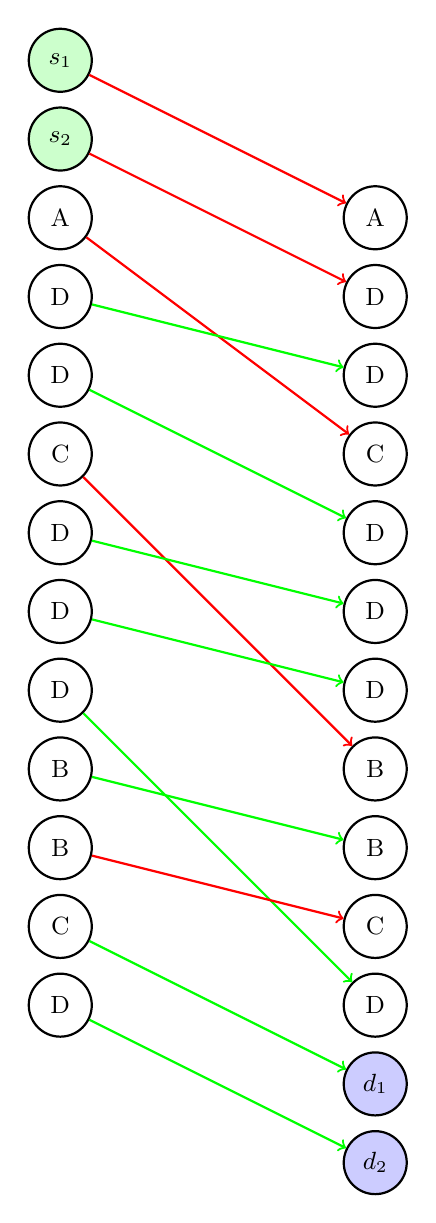
\begin{tikzpicture}[node distance={10mm}, thick, auto=center, main/.style = {draw, circle}]
                \tikzstyle{main} = [circle, draw, minimum size=0.8cm, font=\small]
                \tikzstyle{source} = [circle, draw, minimum size=0.8cm, font=\small, fill=green!20]
                \tikzstyle{dest} = [circle, draw, minimum size=0.8cm, font=\small, fill=blue!20]

                % Source nodes (left column, green background)
                \node[source] (s1) {$s_1$};
                \node[source] (s2) [below of=s1] {$s_2$};
                
                % Tree nodes (left column, red border)
                \node[main] (t1) [below of=s2] {A};
                \node[main] (t2) [below of=t1] {D};
                \node[main] (t3) [below of=t2] {D};
                \node[main] (t4) [below of=t3] {C};
                \node[main] (t5) [below of=t4] {D};
                \node[main] (t6) [below of=t5] {D};
                \node[main] (t7) [below of=t6] {D};
                \node[main] (t8) [below of=t7] {B};
                \node[main] (t9) [below of=t8] {B};
                \node[main] (t10) [below of=t9] {C};
                \node[main] (t11) [below of=t10] {D};
                
                % Tree nodes (right column, red border)
                \node[main] (r1) [right of=t1, xshift=3cm] {A};
                \node[main] (r2) [below of=r1] {D};
                \node[main] (r3) [below of=r2] {D};
                \node[main] (r4) [below of=r3] {C};
                \node[main] (r5) [below of=r4] {D};
                \node[main] (r6) [below of=r5] {D};
                \node[main] (r7) [below of=r6] {D};
                \node[main] (r8) [below of=r7] {B};
                \node[main] (r9) [below of=r8] {B};
                \node[main] (r10) [below of=r9] {C};
                \node[main] (r11) [below of=r10] {D};
                
                % Destination nodes (right column, blue background)
                \node[dest] (d1) [below of=r11] {$d_1$};
                \node[dest] (d2) [below of=d1] {$d_2$};
                
                \draw[red, ->] (s1) -- (r1);
                \draw[red, ->] (s2) -- (r2);
                \draw[red, ->] (t1) -- (r4);
                \draw[green, ->] (t2) -- (r3);
                \draw[green, ->] (t3) -- (r5);
                \draw[red, ->] (t4) -- (r8);
                \draw[green, ->] (t5) -- (r6);
                \draw[green, ->] (t6) -- (r7);
                \draw[green, ->] (t7) -- (r11);
                \draw[green, ->] (t8) -- (r9);
                \draw[red, ->] (t9) -- (r10);
                \draw[green, ->] (t10) -- (d1);
                \draw[green, ->] (t11) -- (d2);
            \end{tikzpicture} \\
        (a) & (b) \\
        \end{tabular}
        \caption[Reduction full example]{Example of a reduction for the tree in \cref{fig:original_tree}. In (a), we have the resulting bipartite graph constructed. In (b), we have the resulting perfect matching for the graph in (a). Green edges weigh $0$, while red edges weigh $1$.}
        \label{fig:reduction_example}
    \end{figure}
\end{example}

\subsection{Heuristics and Improvements}
Some changes can be made to the reduction in order to optimize it and to reduce the number of edges in the bipartite graph. Here are some of the improvements that can be made.
    
\begin{lemma}[Sources' edges optimization] \label{lemma:sources_optimization}
    The sources' edges can be optimized by connecting each source only to the smallest node in $\treeset{2}$ that is not connected to any other source.
\end{lemma}

\begin{proof}
    Since the source nodes are needed to distinguish the chains as starting points, we need that each source is connected to exactly one node in $\treeset{2}$. Having the sources connected to the first $p$ nodes with distinct equivalence classes in $\treeset{2}$ is not necessary since it allows us just to invert the chains starting from each source, and so it is redundant. 

    Moreover, Hall's condition $|N(W)| \geq |W|$ still holds for any subset $W \subseteq V_1$ in the optimized graph. This follows trivially from the fact that case 1 of \cref{lemma:matching_existence} still guarantees that $|N(W)| \geq |W|$ for any subset $W \subseteq \sourceset$.
\end{proof}

\begin{example}
    Consider the bipartite graph shown in \cref{fig:source_optimization}. The red solid arrows represent edges with weight 1, while the red dashed arrows represent edges that can be optimized away according to \cref{lemma:sources_optimization}.

    In this example, we can observe the application of the optimization rule:
    \begin{itemize}
        \item The first tree node $A$ has a solid edge to the first destination node $A$ and a dashed edge to destination node $B$ to be removed. This since source $s_1$ is already connected to node $A$.
        \item Similarly, the second source node $s_2$ has a dashed edge to the first destination node $A$, which can be removed because $s_1$ is already connected to node $A$ with the same weight.
    \end{itemize}

    After applying the optimization, only the solid edges remain, resulting in a reduced bipartite graph that maintains the same optimal matching cost while having fewer edges to consider during the matching algorithm.
    \begin{figure}[H]
        \centering
        \tikzset{main/.style = {draw, circle, thick, minimum size=8mm, inner sep=0pt}}
        \begin{tikzpicture}[node distance=10mm, auto=center]
            \tikzstyle{main} = [circle, draw, minimum size=0.8cm, font=\small]
            \tikzstyle{source} = [circle, draw, minimum size=0.8cm, font=\small, fill=green!20]
            \tikzstyle{dest} = [circle, draw, minimum size=0.8cm, font=\small, fill=blue!20]
            
            % Left column (sources)
            \node[source] (1s) {$s_1$};
            \node[source] (2s) [below of=1s] {$s_2$};
            \node[main] (3s) [below of=2s] {A};
            \node[right=0cm of 3s] {$\cdots$};
            \node[main] (4s) [below of=3s] {A};
            \node[right=0cm of 4s] {$\cdots$};
            \node[main] (5s) [below of=4s] {B};
            \node[right=0cm of 5s] {$\cdots$};
            \node (dots_s) [below of=5s] {\vdots}; % Vertical dots

            % Right column (destinations)
            \node[main] (1d) [right=2.5cm of 3s] {A};
            \node[main] (2d) [below of=1d] {A};
            \node[left=0cm of 2d] {$\cdots$};
            \node[main] (3d) [below of=2d] {B};
            \node[left=0cm of 3d] {$\cdots$};
            \node (dots_d) [below of=3d] {\vdots}; % Vertical dots

            % Arrows
            \draw[red, ->] (1s) -- (1d);
            \draw[red, dashed, ->] (1s) -- (3d);
            \draw[red, dashed, ->] (2s) -- (1d);
            \draw[red, ->] (2s) -- (3d);
        \end{tikzpicture}
        \caption{Bipartite graph after applying Sources' edges optimization. Dashed edges from the original graph have been removed according to \cref{lemma:sources_optimization}, reducing the number of edges while preserving optimality. Red edges have weight $1$.}
        \label{fig:source_optimization}
    \end{figure}
\end{example}

This will reduce the number of edges coming from the sources from $p^2$ to $p$.

\begin{lemma}[Tree nodes' edges optimization 1] \label{lemma:tree_optimization_1}
    The tree nodes' edges can be optimized by removing the edges of the nodes in $\treeset{1}$ that are connected to nodes in $\treeset{2}$ already linked to a source node in $V_1$.
\end{lemma}

\begin{proof}
    This optimization follows directly from \cref{lemma:sources_optimization}.
    From \cref{def:matching} we know that a matching $M \in E$ is a collection of edges such that every vertex of $V$ is incident to at most one edge of $M$. In other words, a matching is a set of edges such that no two edges share a common vertex. Given that, in all the solutions to the problem, all sources will be connected to exactly one node in $\treeset{2}$. Therefore, we can remove the edges of the nodes in $\treeset{1}$ that are connected to nodes in $\treeset{2}$ already linked to a source node in $V_1$ since they will not be part of the final matching.
\end{proof}

\begin{example}
    Consider the bipartite graph shown in \cref{fig:tree_optimization_1}. The red arrows represent edges with weight $1$, while green arrows represent edges with weight $0$. Dashed edges represent edges that can be optimized away according to \cref{lemma:tree_optimization_1}.

    In particular, in \cref{fig:tree_optimization_1}, we can observe that the dashed edge from the first node $A$ in $\treeset{1}$ can be optimized away since it is connected to $B$ in $\treeset{2}$, which is already linked to a source node in $V_1$.
    \begin{figure}[H]
        \tikzset{main/.style = {draw, circle, thick, minimum size=8mm, inner sep=0pt}}
        \centering
        \begin{tikzpicture}[node distance=10mm, auto=center]
            \tikzstyle{main} = [circle, draw, minimum size=0.8cm, font=\small]
            \tikzstyle{source} = [circle, draw, minimum size=0.8cm, font=\small, fill=green!20]
            \tikzstyle{dest} = [circle, draw, minimum size=0.8cm, font=\small, fill=blue!20]
            
            % Left column (sources)
            \node[source] (1s) {$s_1$};
            \node[source] (2s) [below of=1s] {$s_2$};
            \node[main] (3s) [below of=2s] {A};
            \node[main] (4s) [below of=3s] {A};
            \node[right=0cm of 4s] {$\cdots$};
            \node[main] (5s) [below of=4s] {B};
            \node[right=0cm of 5s] {$\cdots$};
            \node[main] (6s) [below of=5s] {C};
            \node[right=0cm of 6s] {$\cdots$};
            \node (dots_s) [below of=6s] {\vdots}; % Vertical dots

            % Right column (destinations)
            \node[main] (1d) [right=2.5cm of 3s] {A};
            \node[main] (2d) [below of=1d] {A};
            \node[main] (3d) [below of=2d] {B};
            \node[left=0cm of 3d] {$\cdots$};
            \node[main] (4d) [below of=3d] {C};
            \node[left=0cm of 4d] {$\cdots$};
            \node (dots_d) [below of=4d] {\vdots}; % Vertical dots

            % Arrows
            \draw[red, ->] (1s) -- (1d);
            \draw[red, ->] (2s) -- (3d);
            \draw[green, ->] (3s) -- (2d);
            \draw[red, ->, dashed] (3s) -- (3d);
            \draw[red, ->] (3s) -- (4d);

        \end{tikzpicture}
        \caption{Bipartite graph after applying tree nodes' edges optimization 1. Dashed edges from the original graph have been removed according to \cref{lemma:tree_optimization_1}, reducing the number of edges while preserving optimality. Red edges have weight $1$, while green edges have weight $0$.}
        \label{fig:tree_optimization_1}
    \end{figure}
\end{example}

This will reduce the number of edges by a factor of $p-1$.

\begin{lemma}[Tree nodes' edges optimization 2] \label{lemma:tree_optimization_2}
    Edges of nodes in $\treeset{1}$ can be optimized by removing the edges with weight $1$ starting from a node $u \in \treeset{1}$ to a node $v \in \treeset{2}$ if the node $u$ has another edge with weight $0$ connected to a node $z \in \treeset{2}$ such that $z \prec v$ in the ordering of the nodes.
\end{lemma}

\begin{proof}
    Let $M$ be any perfect matching. Suppose $M$ contains an edge $(u, v)$ that satisfies the conditions of the lemma, i.e., $u \in \treeset{1}$, $v \in \treeset{2}$, $w(u,v) = 1$, and there exists an edge $(u, z)$ with $w(u,z) = 0$ for some $z \in \treeset{2}$ with $z \prec v$.

    We will show that this edge $(u,v)$ is not necessary for an optimal solution. Since $M$ is a perfect matching, $z$ must be matched with some node $u' \in \treeset{1}$, so $(u',z) \in M$. Note that $u' \neq u$ and that $u' \prec z$ for \cref{lemma:greater_nodes}.

    Consider an alternative matching $M' = (M \setminus \{(u,v), (u',z)\}) \cup \{(u,z), (u'',v)\}$. This is a valid perfect matching where $u$ is matched with $z$, and $u'' \in \treeset{1}$ is matched with $v$. By construction and from \cref{lemma:greater_nodes} we know that $u \prec u' \preceq u'' \prec v$.
    
    The weight of this new matching is $W(M') = W(M) - w(u,v) - w(u',z) + w(u,z) + w(u'',v)$.
    By substituting the known weights $w(u,v)=1$ and $w(u,z)=0$, we get:
    $W(M') = W(M) - 1 - w(u',z) + 0 + w(u'',v) = W(M) + (w(u'',v) - w(u',z)) - 1$.

    The construction of the graph ensures that for any node $u'' \in \treeset{1}$, the cost of connecting to $v$ is either the same or one greater than connecting to a preceding node $z$. That is, $w(u'',v) - w(u',z) \in \{-1, 1\}$. This property arises from the problem reduction, where moving to a subsequent node in the ordering can at most increment the cost by one.
    
    Therefore, $w(u'',v) - w(u',z) \le 1$, which implies $W(M') \leq W(M)$. Thus, the edge $(u,v)$ can be removed from the graph without affecting the weight of the optimal solution.

    Finally, we need to prove that \cref{lemma:matching_existence} still holds. The proof follows from showing that the two fundamental neighborhood properties remain valid after edge removal:
    \begin{enumerate}[leftmargin=25pt]
        \item \cref{lemma:distinct_neighborhoods} remains valid because it relies on the fact that each node $u_i \in \treeset{1}$ is connected to $v_{i+1} \in \treeset{2}$. The edge $(u,v)$ we remove cannot be this critical edge $(u_i,v_{i+1})$ since, by our optimization condition, there exists a node $z \prec v$ connected to $u$ with weight 0; the edge $(u_i,v_{i+1})$ is always the first valid connection for $u_i$ in the ordering. Therefore, $v$ cannot be $v_{i+1}$ for the node $u$.
        \item \cref{lemma:distinct_neighborhoods_2} is preserved because it concerns edges between nodes of the same equivalence class. Our optimization only removes an edge when there exists a better alternative to a preceding node, meaning that the same-class connectivity pattern is unaffected by this edge removal.
        \item The edge removal does not affect source and destination nodes' connections, as we only remove tree node edges.
    \end{enumerate}

    Since both \cref{lemma:distinct_neighborhoods,lemma:distinct_neighborhoods_2} remain valid and the source and destination connectivity is preserved, all conditions required by \cref{lemma:matching_existence} continue to hold, ensuring the existence of a perfect matching in the optimized graph.

    \alessio{La questione è che: se da un nodo con valore 1 voglio connettermi ad un nodo con valore 3, ma prima c'è un altro nodo con valore 1, tanto vale pasó che comunque ci sarà un collegamento tra quello nuovo e li 3 (da dimostrare). In questo modo, prendendo quel nodo, il costo della mia catena aumenta di 0, quindi non peggiora, e il coto di un altra catena potrebbe non aumentare, quindi togliamo una scelta ovviamente errata.} \davide{ho provato a renderla più generale. così mi sembra funzionare}
\end{proof}

\begin{example}
    Consider the bipartite graph in \cref{fig:tree_optimization_2}. The red arrows represent edges with weight $1$, while green arrows represent edges with weight $0$. Dashed edges represent edges that can be optimized away according to \cref{lemma:tree_optimization_2}.

    In this case, we can observe the application of the optimization rule: The edge $(A, C)$ is removed from the graph, as it is not necessary for an optimal solution. This is because the node $A$ has another edge with weight $0$ connected to a node $B$ with $B \prec C$.
    \begin{figure}[H]
        \tikzset{main/.style = {draw, circle, thick, minimum size=8mm, inner sep=0pt}}
        \centering
        \begin{tikzpicture}[node distance=10mm, auto=center]
            \tikzstyle{main} = [circle, draw, minimum size=0.8cm, font=\small]
            \tikzstyle{source} = [circle, draw, minimum size=0.8cm, font=\small, fill=green!20]
            \tikzstyle{dest} = [circle, draw, minimum size=0.8cm, font=\small, fill=blue!20]

            % Left column (tree nodes)
            \node (dots_s_top) {\vdots};
            \node[main] (3s) [below of=dots_s_top] {A};
            \node[main] (4s) [below of=3s] {B};
            \node[right=0cm of 4s] {$\cdots$};
            \node[main] (5s) [below of=4s] {A};
            \node[right=0cm of 5s] {$\cdots$};
            \node[main] (6s) [below of=5s] {C};
            \node[right=0cm of 6s] {$\cdots$};
            \node (dots_s_bottom) [below of=6s] {\vdots};

            % Right column (destinations)
            \node (dots_d_top) [right=2.5cm of dots_s_top] {\vdots};
            \node[main] (1d) [below of=dots_d_top] {A};
            \node[left=0cm of 1d] {$\cdots$};
            \node[main] (2d) [below of=1d] {B};
            \node[left=0cm of 2d] {$\cdots$};
            \node[main] (3d) [below of=2d] {A};
            \node[left=0cm of 3d] {$\cdots$};
            \node[main] (4d) [below of=3d] {C};
            \node[left=0cm of 4d] {$\cdots$};
            \node (dots_d_bottom) [below of=4d] {\vdots};

            % Arrows
            \draw[red, ->] (3s) -- (2d);
            \draw[red, dashed, ->] (3s) -- (4d);
            \draw[green, ->] (3s) -- (3d);
        \end{tikzpicture}
        \caption{Bipartite graph after applying tree nodes' edges optimization 2. Dashed edges from the original graph have been removed according to \cref{lemma:tree_optimization_2}, reducing the number of edges while preserving optimality. Red edges have weight $1$, while green edges have weight $0$.}
        \label{fig:tree_optimization_2}
    \end{figure}
\end{example}

\begin{comment}
In \cref{fig:heuristics_example}-(b), we can see the resulting bipartite graph for the example shown in the previous section after the optimizations.

\begin{figure}[H]
    \centering
    \begin{tabular}{cc}
        \begin{tikzpicture}[node distance={10mm}, thick, auto=center, main/.style = {draw, circle}]
            \node[main] (1s) {$s_1$};
            \node[main] (2s) [below of=1s] {$s_2$};
            \node[main] (3s) [below of=2s] {$1$};
            \node[main] (4s) [below of=3s] {$2$};
            \node[main] (5s) [below of=4s] {$1$};
            \node[main] (6s) [below of=5s] {$3$};
            \node[main] (7s) [below of=6s] {$1$};
            \node[main] (8s) [below of=7s] {$2$};
            \node[main] (9s) [below of=8s] {$2$};
            \node[main] (1d) [right=3cm of 3s] {$1$};
            \node[main] (2d) [below of=1d] {$2$};
            \node[main] (3d) [below of=2d] {$1$};
            \node[main] (4d) [below of=3d] {$3$};
            \node[main] (5d) [below of=4d] {$1$};
            \node[main] (6d) [below of=5d] {$2$};
            \node[main] (7d) [below of=6d] {$2$};
            \node[main] (8d) [below of=7d] {$d_1$};
            \node[main] (9d) [below of=8d] {$d_2$};

            \draw[black, dashed, ->] (1s) -- (1d);
            \draw[green, dashed, ->] (1s) -- (2d);
            \draw[green, dashed, ->] (2s) -- (1d);
            \draw[black, dashed, ->] (2s) -- (2d);
            \draw[blue, dashed, ->] (3s) -- (2d);
            \draw[red, dashed, ->] (3s) -- (4d);
            \draw[black, ->] (3s) -- (3d);
            \draw[black, dashed, ->] (4s) -- (3d);
            \draw[black, dashed, ->] (4s) -- (4d);
            \draw[black, ->] (4s) -- (6d);
            \draw[black, dashed, ->] (5s) -- (4d);
            \draw[black, ->] (5s) -- (5d);
            \draw[red, dashed, ->] (5s) -- (6d);
            \draw[black, dashed, ->] (6s) -- (5d);
            \draw[black, dashed, ->] (6s) -- (6d);
            \draw[black, ->] (6s) -- (8d);
            \draw[black, ->] (6s) -- (9d);
            \draw[black, dashed, ->] (7s) -- (6d);
            \draw[black, ->] (7s) -- (8d);
            \draw[black, ->] (7s) -- (9d);
            \draw[black, ->] (8s) -- (7d);
            \draw[black, ->] (9s) -- (8d);
            \draw[black, ->] (9s) -- (9d);
        \end{tikzpicture} &
        \begin{tikzpicture}[node distance={10mm}, thick, auto=center, main/.style = {draw, circle}]
            \node[main] (1s) {$s_1$};
            \node[main] (2s) [below of=1s] {$s_2$};
            \node[main] (3s) [below of=2s] {$1$};
            \node[main] (4s) [below of=3s] {$2$};
            \node[main] (5s) [below of=4s] {$1$};
            \node[main] (6s) [below of=5s] {$3$};
            \node[main] (7s) [below of=6s] {$1$};
            \node[main] (8s) [below of=7s] {$2$};
            \node[main] (9s) [below of=8s] {$2$};
            \node[main] (1d) [right=3cm of 3s] {$1$};
            \node[main] (2d) [below of=1d] {$2$};
            \node[main] (3d) [below of=2d] {$1$};
            \node[main] (4d) [below of=3d] {$3$};
            \node[main] (5d) [below of=4d] {$1$};
            \node[main] (6d) [below of=5d] {$2$};
            \node[main] (7d) [below of=6d] {$2$};
            \node[main] (8d) [below of=7d] {$d_1$};
            \node[main] (9d) [below of=8d] {$d_2$};

            \draw[black, dashed, ->] (1s) -- (1d);
            \draw[black, dashed, ->] (2s) -- (2d);
            \draw[black, ->] (3s) -- (3d);
            \draw[black, dashed, ->] (4s) -- (3d);
            \draw[black, dashed, ->] (4s) -- (4d);
            \draw[black, ->] (4s) -- (6d);
            \draw[black, dashed, ->] (5s) -- (4d);
            \draw[black, ->] (5s) -- (5d);
            \draw[black, dashed, ->] (6s) -- (5d);
            \draw[black, dashed, ->] (6s) -- (6d);
            \draw[black, ->] (6s) -- (8d);
            \draw[black, ->] (6s) -- (9d);
            \draw[black, dashed, ->] (7s) -- (6d);
            \draw[black, ->] (7s) -- (8d);
            \draw[black, ->] (7s) -- (9d);
            \draw[black, ->] (8s) -- (7d);
            \draw[black, ->] (9s) -- (8d);
            \draw[black, ->] (9s) -- (9d);
        \end{tikzpicture} \\
    (a) & (b) \\
    \end{tabular}
    \caption[Reduction heuristics example]{Example of a reduction for the sorted nodes' equivalency classes $E = \{1,2,1,3,1,2,2\}$ applying also the heuristics shown. In (a), the edges removed are shown in green for \cref{lemma:sources_optimization}, blue for \cref{lemma:tree_optimization_1}, and red for \cref{lemma:tree_optimization_2}. In (b), we have the resulting bipartite graph after the heuristics are applied. Dashed edges weigh $1$, while solid edges weigh $0$. \alessio{Invertirei la notazione degli archi: dashed (semi-trasparente) logicamente ha peso 0, mentre solid (si vede bene) ha peso 1.}}
    \label{fig:heuristics_example}
\end{figure}
\end{comment}

\subsection{Moving to Maximum weight perfect bipartite matching}
In this section, we will discuss how to slightly modify the reduction process to move from a minimum weight perfect bipartite matching problem to a maximum weight perfect bipartite matching problem. This will be helpful in solving the problem more efficiently by using some known algorithms to solve the maximum weight perfect bipartite matching problem.

\begin{theorem}
    An optimal solution of an instance $\mathcal I$ with $p \leq |E|$ of the \textsc{CHAINS-DIVISION} problem is equivalent to an optimal solution of the Maximum Weight Perfect Bipartite Matching for the instance $r(\mathcal I)$ where $r: \mathcal{I}_{CHAINS-DIVISION} \rightarrow \mathcal{I}_{MWPBM}$ is the reduction function that maps an instance of the \textsc{CHAINS-DIVISION} problem to an instance of the Maximum Weight Perfect Bipartite Matching problem constructed as stated in \cref{def:bip_construction} but with inverted weights (weight $0$ becomes $1$ and weight $1$ becomes $0$).
\end{theorem}

\begin{proof}
    Let $M$ be a perfect matching in the bipartite graph $G$ constructed as stated in \cref{def:bip_construction}. Let $w(M)$ be the sum of the weights of the edges in the matching $M$. From the previous theorem, we know that the optimal solution of the \textsc{CHAINS-DIVISION} problem is equivalent to finding a perfect matching $M$ in $G$ that minimizes $w(M)$.

    Let $G'$ be a bipartite graph constructed as $G$ but with inverted weights (weight $0$ becomes $1$ and weight $1$ becomes $0$). Let $M'$ be a perfect matching in $G'$ and let $w'(M')$ be the sum of the weights of the edges in the matching $M'$. Let $k$ be the number of edges in the matching.

    We can see that for any matching $M$ in $G$:
    \[ w'(M) = k - w(M) \]

    This means that maximizing $w'(M)$ is equivalent to minimizing $w(M)$. Therefore, finding the maximum weight perfect matching in $G'$ is equivalent to finding the minimum weight perfect matching in $G$, which in turn is equivalent to finding the optimal solution of the \textsc{CHAINS-DIVISION} problem.
\end{proof}
